\documentclass[a4paper,titlepage]{article}

\usepackage{fullpage}
\usepackage{fontenc}
\usepackage{mathptmx}
\usepackage{hyperref}
\usepackage{tikz}
\usepackage{graphicx}
\usepackage{float}
\usepackage{parskip}

\renewcommand{\contentsname}{Contenidos}

\hypersetup{
    colorlinks=true,
    linkcolor=blue,
    filecolor=magenta,
    urlcolor=blue,
}

\urlstyle{same}

\begin{document}

\title{POO - MasterMind}
\author{Moltrasio, Mauro Ezequiel}
\date{}

\maketitle
\tableofcontents

\section{Introducción}

El propósito de este documento es detallar el proceso de diseño e
implementación de un programa que permitirá a un usuario jugar un juego de
MasterMind contra el ordenador. Se describirá primero el diseño de la
aplicación acorde a los requisitos especificados, se proveerá un diagrama de
clases UML de alto nivel y finalmente se explicarán algunos detalles
particulares de la aplicación con el propósito de simplificar el entendimiento
de la misma.

\section{Diseño de la solución}

Las reglas del juego MasterMind se pueden encontrar en el siguiente enlace:
\url{https://www.infotecnovision.com/Multimedia/REGLAS-DEL-MASTERMIND.pdf}.

Siguiendo la descripción de ese documento, podemos ver que a grandes rasgos
necesitaremos un tablero y clavijas de color, empecemos por las clavijas.

\subsection{Las clavijas}

Las clavijas son el componente más básico del juego, cómo las definamos
afectará el diseño de nuestra aplicación en su totalidad. Siendo que las
clavijas tienen un cierto rango de colores que pueden pertenecer y cada
clavija sólo puede ser de un solo color, la forma correcta de representarlas
sería definir un enum de colores y hacer que las clavijas tomen uno de estos
valores como parte de su constructor, bloqueando el color como una
caraterística de sólo lectura.

Adelantando un poco, al empezar con esta implementación se encontró que hay dos
tipos de clavijas que deben distinguirse:
\begin{itemize}
    \item Clavijas jugables
    \item Clavijas de clave (usadas para dar pistas al jugador)
\end{itemize}

Resultó claro entonces que se debía hacer una especialización para asegurarnos
que un usuario no pueda utilizar una clavija clave como una parte del juego, ni
que el ordenador utilice erróneamente una clavija jugable como clave. Para esto
se decidió crear una interface Color y separar el enum en dos:
\begin{itemize}
    \item PlayableColor: Colores que el usuario usa para jugar y componen el
        código secreto.
    \item KeyColor: Utilizados por el ordenador para dar pistas sobre el
        código secreto.
\end{itemize}

Haciendo esta distinción y haciendo que las clavijas acepten un Color, podemos
agrupar esas clavijas en componentes de niveles más alto. Veremos más adelante
que se utilizó composición para definir qué clavijas son aceptadas en qué
sectores del tablero.

\subsection{El tablero}

Contrario a las clavijas, el tablero será el componente de más alto nivel en
nuestra aplicación. Este será responsable de tomar las jugadas del usuario,
compararlas con el código secreto, proveer pistas y permitir una representación
amigable del juego para el usuario.

Como se mencionó en la sección anterior, la solución final utiliza composición
para agrupar componentes en esta clase. Si comenzamos con la visión global del
tablero:

\begin{figure}[H]
    \centering
    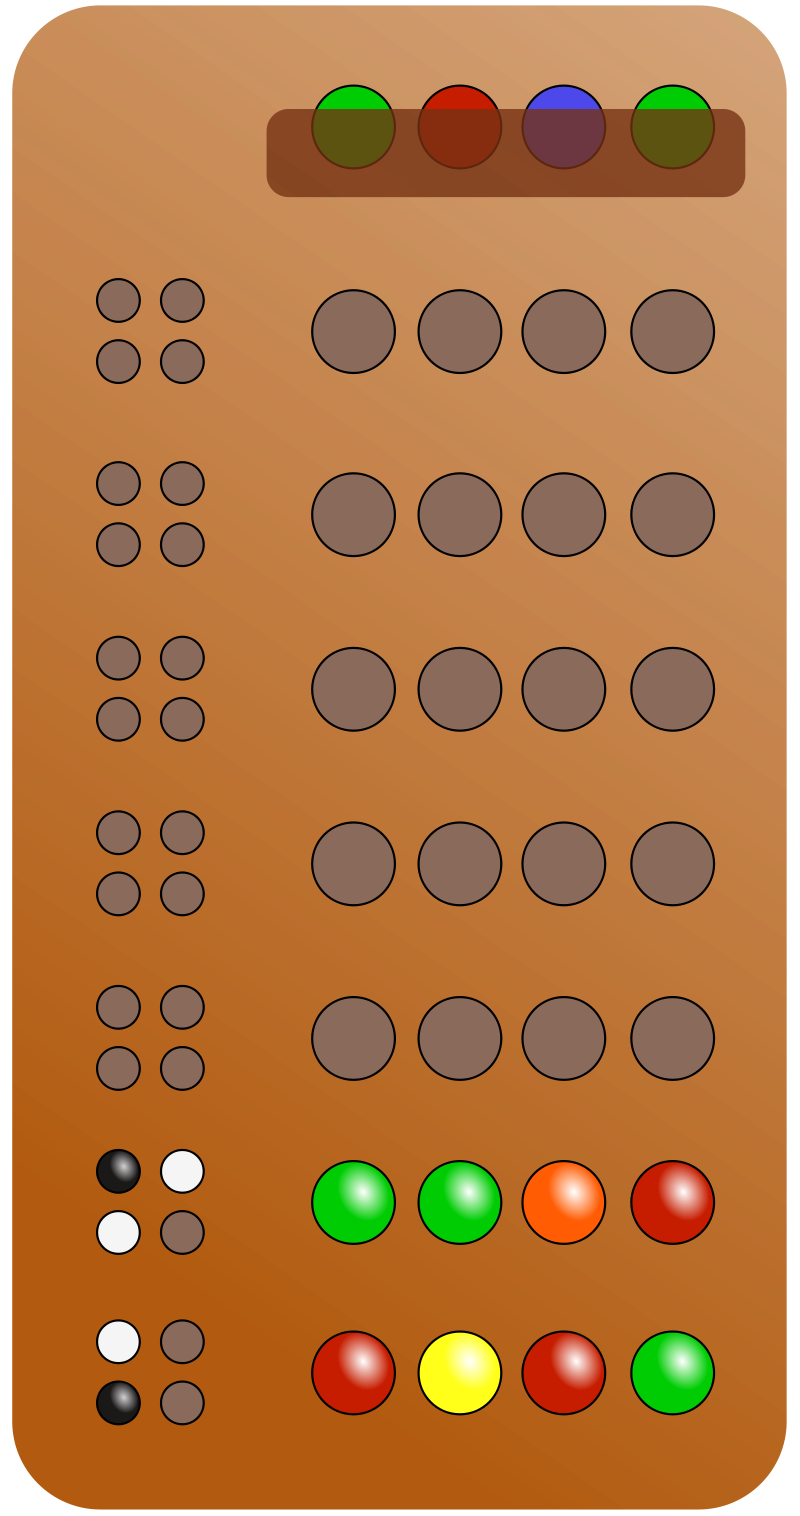
\includegraphics[scale=0.2]{imgs/Mastermind.png}
\end{figure}

Podemos ver que hay tres sectores bien definidos:
\begin{itemize}
    \item Un sector con el código secreto.
    \item Un sector de juego para que el usuario pueda hacer sus jugadas.
    \item Un sector para que el ordenador provea pistas para cada jugada.
\end{itemize}

También podemos apreciar que las clavijas se agrupan por filas por lo que,
una vez definamos este componente, los sectores en el tablero pueden definirse
como arrays de filas para los sectores de juego y pistas, teniendo una fila
adicional para el código secreto.

\section{Diagrama de clases}

Con lo discutido hasta este punto podemos plantear un diagrama de clases como
el siguiente:

\begin{figure}[H]
    \centering
    \scalebox{.6}{
        \input{build/uml.tex}
    }
\end{figure}

Se pueden ver un par de clases más que no se han discutido hasta este punto,
la siguiente sección detallará un poco más sobre estas clases y la interacción
final de toda la aplicación.

\section{Detalles de la implementación}

\subsection{Clases adicionales}

La aplicación iniciará a partir de una clase App, la cual contendrá el método
main. Lo primero que realizará el programa al iniciar es instanciar un objeto
de la clase UserInterface, este será responsable de mostrar texto al usuario y
tomar datos de entrada que este realice para jugar.
Se pide al usuario que ingrese el número de partidas que desea jugar y se
comenzará a jugar inmediatamente.
A efectos prácticos, cada tablero que se cree en el programa será un nuevo
juego, por lo que el lazo de juego es sencillo:

\begin{enumerate}
    \item Instanciar el nuevo tablero (el código secreto se genera con el tablero).
    \item Imprimir el tablero.
    \item Pedir al usuario que genere una fila para probar contra el código secreto.
    \item Mientras no se haya adivinado el código y queden intentos, volver al punto 2.
    \item Una vez terminado el juego, añadir la puntuación de este juego a la global.
    \item Cuando se hayan jugado todas las partidas, imprimir la puntuación final.
\end{enumerate}

\subsection{Modos de representación}

Por defecto, la aplicación utiliza caracteres UTF-16 y códigos de terminal
Unix para representar el tablero como se muestra a continuación:

\begin{figure}[H]
    \centering
    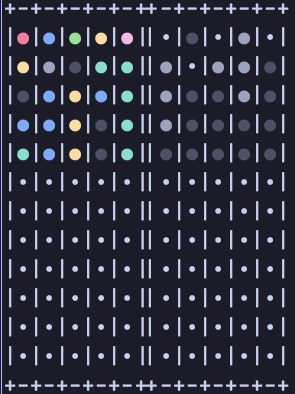
\includegraphics[scale=0.5]{imgs/MastermindColor.png}
\end{figure}

Si se desea jugar en una terminal con la que este tipo de salida no es
compatible, se puede utilizar la variable de entorno
MASTERMIND{\_}USE{\_}COLORS con el valor false para que la aplicación
utilice texto plano, como se muestra a continuación:

\begin{figure}[H]
    \centering
    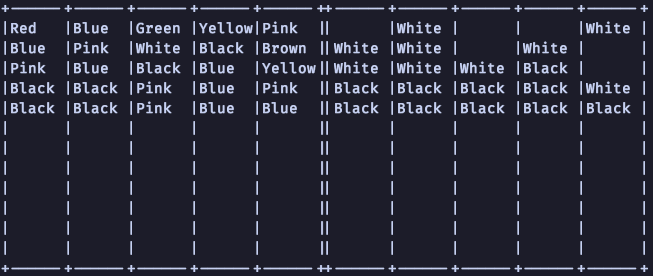
\includegraphics[scale=0.5]{imgs/MastermindWords.png}
\end{figure}

\section{Referencia}
\begin{itemize}
    \item Wikipedia: https://es.wikipedia.org/wiki/Mastermind
\end{itemize}

\end{document}
